\documentclass[12pt]{article}

\usepackage{float}
\usepackage{xcolor}
\usepackage{amsmath}
\usepackage{amsfonts}
\usepackage{listings} 
\usepackage{geometry} 
\usepackage{graphicx}
\usepackage[utf8]{inputenc} 
\geometry{a4paper, margin=1in}

\lstset{
    language=Python,
    keywordstyle=\color{blue}\bfseries,
    stringstyle=\color{red},
    commentstyle=\color{green!60!black},
    breaklines=true
}

\begin{document}

\begin{center}
    \textbf{\large ME 4511: Fluid Mechanics II} \\
    \vspace{0.5em}
    \textbf{Assignment 1} \\
    \vspace{0.5em}
    \textit{Abdullah al Azmi, 220011230}
    \vspace{1em}
\end{center}

\noindent \textbf{Q1} Here, the velocity field is:

\begin{align}
    u &= a(x^2-y^2) \\
    v &= -2axy
\end{align}

\begin{enumerate}

    \item[\textbf{(i)}] For a 2D flow, a stream function $\psi$ exists if the flow is incompressible, which means that the continuity equation must be satisfied:
    
    \begin{equation*}
        \frac{\partial u}{\partial x} + \frac{\partial v}{\partial y} = 0
    \end{equation*}

    Now, calculating the partial derivatives:
    
    \begin{equation*}
        \frac{\partial u}{\partial x} = \frac {\partial}{\partial x}[a(x^2-y^2)] = 2ax
    \end{equation*}

    \begin{equation*}
        \frac{\partial v}{\partial y} = \frac{\partial}{\partial y}[-2axy] = -2ax
    \end{equation*}
    
    Substituting into the continuity equation:
    
    \begin{equation*}
        2ax + (-2ax) = 0
    \end{equation*}
    
    Since, the continuity equation is satisfied, a stream function does exist for this flow.

    \vspace{1em}
    
    \item[\textbf{(ii)}] Now, we obtain an expression for stream function $\psi$ and velocity potential $\phi$.

    \vspace{1em}

    Before that we have to verify whether a velocity potential exists for this 2D incompressible, and steady flow or not. A velocity potential $\phi$ exists if the flow is irrotational, which means that the z-component of vorticity $\omega$ must be zero:

    \begin{equation*}
        \omega = \frac{\partial v}{\partial x} - \frac{\partial u}{\partial y}
    \end{equation*}

    Calculating the partial derivatives:
    \begin{equation*}
        \frac{\partial v}{\partial x} = \frac{\partial}{\partial x}[-2axy] = -2ay
    \end{equation*}

    \begin{equation*}
        \frac{\partial u}{\partial y} = \frac{\partial}{\partial y}[a(x^2-y^2)] = -2ay
    \end{equation*}

    Substituting into the vorticity equation:

    \begin{equation*}
        \omega = -2ay - (-2ay) = 0
    \end{equation*}

    Since the vorticity is zero, the flow is irrotational, and thus a velocity potential $\phi$ exists for this flow.

    \vspace{1em}
    
    \textit{\textbf{a.} Stream Function ($\psi$):} By definition, we know that $u = \frac{\partial \psi}{\partial y}$ and $v = -\frac{\partial \psi}{\partial x}$
    
    \begin{equation*}
        \frac{\partial \psi}{\partial y} = a(x^2-y^2) \implies \psi = \int a(x^2-y^2)dy = ax^2y-\frac{ay^3}{3} + f(x)
    \end{equation*}

    To find $f(x)$, we use the other definition of stream function:
    \begin{equation*}
        -\frac{\partial \psi}{\partial x} = -\frac{\partial}{\partial x}\left(ax^2y-\frac{ay^3}{3} + f(x)\right) = -2axy + f'(x)
    \end{equation*}

    Setting this equal to $v$:
    
    \begin{equation*}
        -2axy + f'(x) = -2axy \implies f'(x) = 0 \implies f(x) = c
    \end{equation*}

    Therefore, the stream function is:

    \begin{equation*}
        \psi = a\left(x^2y - \frac{y^3}{3}\right) + c
    \end{equation*}

    \textit{\textbf{b.} Velocity Potential ($\phi$):} By definition, we also know that $u=\frac{\partial \phi}{\partial x}$ and $v=\frac{\partial \phi}{\partial y}$

    \begin{equation*}
        \frac{\partial \phi}{\partial x} = a(x^2-y^2) \implies \phi=\int a(x^2-y^2)dx = a\left(\frac{x^3}{3}-xy^2\right) + g(y)
    \end{equation*}

    To find $g(y)$, we use the other definition of velocity potential:

    \begin{equation*}
        \frac{\partial \phi}{\partial y} = \frac{\partial}{\partial y}\left(a\left(\frac{x^3}{3}-xy^2\right) + g(y)\right) = -2axy + g'(y)
    \end{equation*}

    Setting this equal to $v$:

    \begin{equation*}
        -2axy + g'(y) = -2axy \implies g'(y) = 0 \implies g(y) = c
    \end{equation*}

    Therefore, the velocity potential is:

    \begin{equation*}
        \phi = a\left(\frac{x^3}{3}-xy^2\right) + c
    \end{equation*}

    \vspace{1em}

    \item[\textbf{(iii)}] Plot of Stream Function for $C$ varying from -230 to 230 and $a=1$ is shown in Figure~\ref{fig:stream_function}:
    
    \begin{figure}[H]
        \centering
        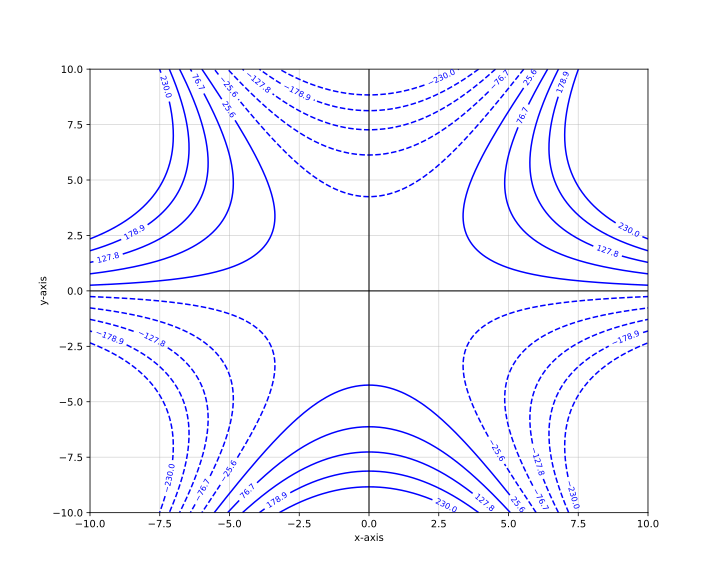
\includegraphics[width=1\textwidth]{figures/stream_function_plot.pdf}
        \caption{Stream Function Contours for $C$ varying from -230 to 230}
        \label{fig:stream_function}
    \end{figure}
    
    \vspace{1em}

    Python code used to generate the plot is as follows:
    
    \begin{lstlisting}[language=Python, breaklines=true, keywordstyle=\color{blue}\bfseries, stringstyle=\color{red}]

    import numpy as np
    import matplotlib.pyplot as plt
        
    a_val = 1
    c_values = np.linspace(-230, 230, 10)
            
    x = np.linspace(-10, 10, 400)
    y = np.linspace(-10, 10, 400)
    X, Y = np.meshgrid(x, y)
            
    psi = a_val * (X**2 * Y - (Y**3)/3)
            
    plt.figure(figsize=(10, 8))
    contour = plt.contour(X, Y, psi, levels=c_values, colors='blue')
    plt.clabel(contour, inline=True, fontsize=8)
    plt.xlabel('x-axis')
    plt.ylabel('y-axis')
    plt.grid(True, alpha=0.5)
    plt.axhline(0, color='black', lw=1)
    plt.axvline(0, color='black', lw=1)
    plt.savefig('stream_function_plot.svg', format='svg')
    plt.show()

    \end{lstlisting}

\end{enumerate}

\vspace{1.5em}
\hrule
\vspace{1.5em}

\noindent \textbf{Q2} For a \textbf{Rankine Half Body}, the flow is obtained by superposing a uniform flow of speed U in the x-direction, and a point source of strength $m$ at the origin. The stagnation point lies where the uniform flow cancels out the source flow and that point is on the negative x-axis where $\theta = \pi$. Now, evaluating the stream function at the stagnation point:

\begin{equation*}
    \psi_s = U r \sin \theta + \frac{m}{2\pi} \theta
\end{equation*}

Substituting the value of $\theta$:

\begin{equation*}
    \psi_s = U r \sin \pi + \frac{m}{2\pi} (\pi) = 0 + \frac{m}{2} = \frac{m}{2}
\end{equation*}

Thus, the value of the stream function at the stagnation point is $\frac{m}{2}$.

\vspace{1em}

\textbf{Equation of streamline}

\vspace{1em}

The equation of the streamline that passes through the stagnation point can be found by setting the stream function equal to $\psi_s$:

\begin{equation*}
    \psi = U r \sin \theta + \frac{m}{2\pi} \theta = \frac{m}{2}
\end{equation*}

Rearranging the equation and solving for $r$:

\begin{equation*}
    U r \sin \theta = \frac{m}{2} - \frac{m}{2\pi} \theta
\end{equation*}

\begin{equation*}
    r = \frac{\frac{m}{2} - \frac{m}{2\pi} \theta}{U \sin \theta} = \frac{m}{2\pi U} \cdot \frac{\pi - \theta}{\sin \theta}
\end{equation*}

Therefore, the equation of the streamline that passes through the stagnation point is:

\begin{equation*}
    r = \frac{m}{2\pi U} \cdot \frac{\pi - \theta}{\sin \theta}
\end{equation*}

\vspace{1.5em}
\hrule
\vspace{1.5em}

\noindent \textbf{Q3} Image of a fluid flow (water) taken using my own image acquisition system (mobile camera) is shown in Figure~\ref{fig:fluid_flow}:

\begin{figure}[htbp]
    \centering
    \includegraphics[width=0.6\textwidth]{figures/laminar_flow_image_horizontal.jpg}
    \caption{Fluid Flow (Water) Captured from Tap to Basin}
    \label{fig:fluid_flow}
\end{figure}

\begin{enumerate}

    \item [\textbf{(i)}] I have captured the image of flowing water from the tap to the basin. The way I have captured this image is by controlling the knob of the tap by using the hand to have a laminar flow of water. Then, I used my mobile camera to take the picture of the flowing water.
    
    \item [\textbf{(ii)}] The flow is laminar because the water stream appears smooth and orderly without any visible turbulence or chaotic motion, which are characteristic features of laminar flow.

    \item [\textbf{(iii)}] To justify whether the flow is steady or unsteady, I have captured a video of 10 seconds of the same flow and analyzed multiple frames of the video using OpenCV library in python. I positioned 10 virtual markers on the water stream in the video frames and tracked their pixel density over time. I observed that the pixel density of these markers remained almost constant throughout the video frames, indicating that the flow characteristics did not change significantly over time. This consistency in pixel density suggests that the flow is steady, as there are no noticeable fluctuations or variations in the flow pattern over the observed period. The analysis is shown in Figures~\ref{fig:marker_positions} and~\ref{fig:heatmap}.
    
    \begin{figure}[H]
        \centering
        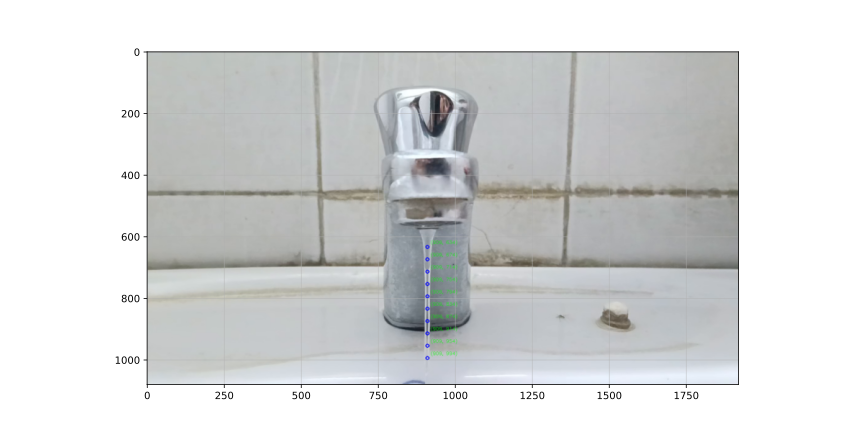
\includegraphics[width=0.8\textwidth]{figures/marked_coordinates_in_first_frame.pdf}
        \caption{Marker Positions on Flow for Pixel Density Tracking}
        \label{fig:marker_positions}
    \end{figure}

    \begin{figure}[H]
        \centering
        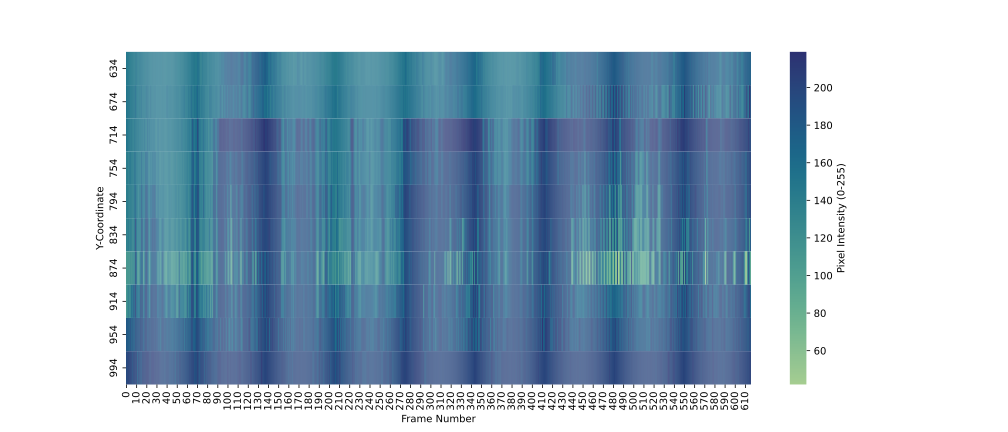
\includegraphics[width=0.8\textwidth]{figures/heatmap_of_different_frame_and_coordinates.pdf}
        \caption{Steady Flow Analysis using Pixel Density Heatmap}
        \label{fig:heatmap}
    \end{figure}

    \item [\textbf{(iv)}] The force I think drive this flow is the pressure difference between the tap and the basin. The water flows from the higher pressure region (tap) to the lower pressure region (basin) due to gravity and the pressure exerted by the water supply system.
    
    \item [\textbf{(v)}] Actually, there was no special reason for choosing this particular flow. I just wanted to capture a simple and common example of fluid flow that is easily observable in everyday life, and I found that the water flowing from a tap to a basin is one of the straightforward examples of fluid flow that I could easily photograph.

\end{enumerate}

\vspace{1.5em}
\hrule
\vspace{1.5em}

\end{document}